% shared preamble of the theory figures (white background, purple / black theme, sans-serif)
\documentclass[tikz,border=8pt]{standalone}
\usepackage[T1]{fontenc}
\usepackage[scaled=0.92]{helvet}
\renewcommand{\familydefault}{\sfdefault}
\usepackage{amsmath,amssymb}
\usepackage[helvet]{sfmath}
\usetikzlibrary{arrows.meta,calc,decorations.pathreplacing,positioning,backgrounds}
\definecolor{ink}{HTML}{1A1A1F}
\definecolor{cohesin}{HTML}{6A3DE8}
\definecolor{condensin}{HTML}{1BAF7A}
\definecolor{fwd}{HTML}{D1303F}      % CTCF pointing right
\definecolor{rev}{HTML}{2B62D9}      % CTCF pointing left
\definecolor{panel}{HTML}{F8F6FD}
\definecolor{panelline}{HTML}{E3DDF5}
\tikzset{
  fiber/.style={line width=2.1pt,ink,line cap=round,line join=round},
  halo/.style={line width=6pt,white,line cap=round},
  lab/.style={font=\small,text=ink},
  note/.style={font=\footnotesize,text=ink!60},
  hd/.style={font=\bfseries\small,text=ink,anchor=west},
  leader/.style={line width=0.6pt,ink!45},
}
% soft panel, numbered badge, heading
\newcommand{\panelbg}[4]{\draw[rounded corners=9pt,fill=panel,draw=panelline,line width=0.9pt] (#1,#2) rectangle (#3,#4);}
\newcommand{\badge}[3]{\fill[ink] (#1,#2) circle (0.21);\node[white,font=\bfseries\footnotesize] at (#1,#2) {#3};}
% CTCF: a protein on the fibre carrying an arrow that gives the motif direction (f = right, r = left)
\newcommand{\protf}[2]{\draw[rounded corners=3.5pt,line width=0.6pt,draw=fwd!65!black,fill=fwd] (#1-0.3,#2-0.19) rectangle (#1+0.3,#2+0.19);
  \draw[white,line width=1.5pt,-{Stealth[length=3.4pt,width=4.4pt]}] (#1-0.15,#2)--(#1+0.16,#2);}
\newcommand{\protr}[2]{\draw[rounded corners=3.5pt,line width=0.6pt,draw=rev!65!black,fill=rev] (#1-0.3,#2-0.19) rectangle (#1+0.3,#2+0.19);
  \draw[white,line width=1.5pt,-{Stealth[length=3.4pt,width=4.4pt]}] (#1+0.15,#2)--(#1-0.16,#2);}
\newcommand{\prot}[3]{\csname prot#3\endcsname{#1}{#2}}
% ring seen at an angle, drawn as a tube (dark outline, light core); back half and front half
\newcommand{\ringpart}[5]{\draw[line width=4.6pt,#3!80!black,line cap=round] ([shift={(#1,#2)}]#4:0.55 and 0.21) arc[start angle=#4,end angle=#5,x radius=0.55,y radius=0.21];
  \draw[line width=2.4pt,#3!55!white,line cap=round] ([shift={(#1,#2)}]#4:0.55 and 0.21) arc[start angle=#4,end angle=#5,x radius=0.55,y radius=0.21];}
\newcommand{\ringback}[3]{\ringpart{#1}{#2}{#3}{180}{0}}
\newcommand{\ringfront}[3]{\ringpart{#1}{#2}{#3}{180}{360}}
% smooth loop whose foot (ring) is at (cx,y0): half-width W, height H, ring colour
\newcommand{\lloop}[5]{%
  \ringback{#1}{#2}{#5}%
  \draw[fiber] (#1-0.3,#2) .. controls (#1-0.3,#2+0.25*#4) and (#1-#3,#2+0.2*#4) .. (#1-#3,#2+0.55*#4)
     .. controls (#1-#3,#2+0.95*#4) and (#1-0.5*#3,#2+#4) .. (#1,#2+#4)
     .. controls (#1+0.5*#3,#2+#4) and (#1+#3,#2+0.95*#4) .. (#1+#3,#2+0.55*#4)
     .. controls (#1+#3,#2+0.2*#4) and (#1+0.3,#2+0.25*#4) .. (#1+0.3,#2);%
  \ringfront{#1}{#2}{#5}}
% gently undulating fibre from x0 to the loop foot at cx (height y0), and from x1
\newcommand{\base}[4]{%
  \draw[fiber] plot[smooth] coordinates {(#1,0.05) (#1+0.35*#3-0.35*#1,-0.05) (#3-1.4,0.04)} .. controls (#3-0.6,0.02) and (#3-0.3,0.05) .. (#3-0.3,#4);
  \draw[fiber] plot[smooth] coordinates {(#2,-0.05) (#2-0.35*#2+0.35*#3,0.05) (#3+1.4,-0.04)} .. controls (#3+0.6,-0.02) and (#3+0.3,0.05) .. (#3+0.3,#4);}
% stop sign for a blocked leg and a leg arrow
\newcommand{\stopbar}[3]{\draw[#3,line width=2.4pt,line cap=round] (#1,#2-0.2)--(#1,#2+0.2);}
\newcommand{\legarrow}[3]{\draw[cohesin,line width=1.6pt,-{Stealth[length=5pt,width=6pt]},line cap=round] (#1,#3)--(#2,#3);}

\begin{document}
\pgfmathsetmacro{\W}{8}                 % map side (cm); 120 bins
\pgfmathsetmacro{\u}{\W/120}
\pgfmathsetmacro{\yM}{-1.7}             % top of the map
\pgfmathsetmacro{\ry}{\yM-12.5*\u}      % row of the fixed anchor (bin 12)
\newcommand{\sw}[3]{% sweeping loop: moving leg at bin #1, line style #2, label #3
  \pgfmathsetmacro{\xb}{#1*\u}\pgfmathsetmacro{\xa}{12*\u}\pgfmathsetmacro{\hh}{0.36*(#1-12)*\u+0.2}%
  \draw[#2,line cap=round] (\xa,0.08) .. controls (\xa,\hh) and (\xb,\hh) .. (\xb,0.08);}
\begin{tikzpicture}
  % contact map
  \node[anchor=north west,inner sep=0] at (0,\yM) {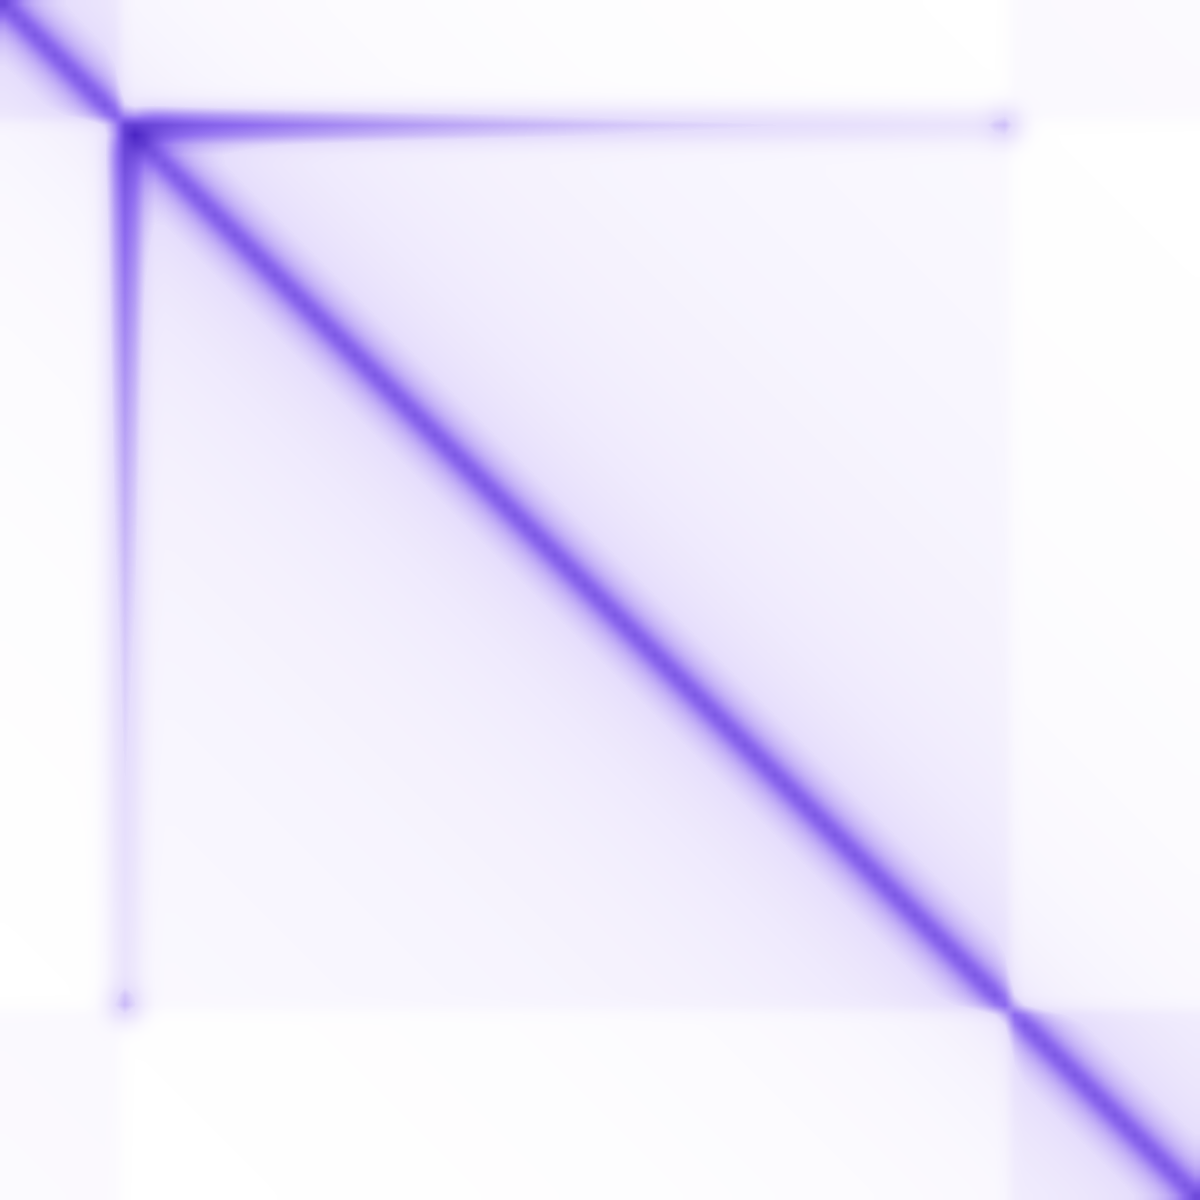
\includegraphics[width=\W cm]{stripe_map.png}};
  \draw[ink!50,line width=0.7pt] (0,\yM) rectangle (\W,{\yM-\W});
  % fibre, CTCF sites and the three snapshots of one loop (older = paler)
  \draw[fiber] (0,0)--(\W,0);
  \pgfmathsetmacro{\pa}{6*\u}\pgfmathsetmacro{\pb}{106*\u}\prot{\pa}{0}{f}\prot{\pb}{0}{r}
  \sw{34}{line width=2pt,cohesin!30}{1}\sw{62}{line width=2.2pt,cohesin!60}{2}\sw{88}{line width=2.6pt,cohesin}{3}
  \legdot{{12*\u}}{0}{cohesin}
  \foreach \b/\k/\c in {34/1/30,62/2/60,88/3/100}{\pgfmathsetmacro{\xx}{\b*\u}%
    \legdot{\xx}{0}{cohesin!\c!white}\node[note,anchor=north] at (\xx,-0.28) {$t_\k$};
    \draw[dashed,ink!30,line width=0.6pt] (\xx,-1.0)--(\xx,{\ry+0.14});
    \fill[white] (\xx,\ry) circle (0.15);\fill[cohesin!\c!white] (\xx,\ry) circle (0.1);}
  \draw[cohesin,line width=1.6pt,-{Stealth[length=5pt,width=6pt]}] ({40*\u},-0.7)--({84*\u},-0.7);
  \node[note,anchor=east] at (-0.2,0) {fibre};
  \node[note,anchor=east] at (-0.2,\yM) {contact map};
  % call-outs
  \pgfmathsetmacro{\xr}{\W+0.5}
  \node[lab,anchor=west,align=left] at (\xr,{\yM+0.2}) {\textbf{stripe}\\[-1pt]{\footnotesize one leg rests at the CTCF,}\\{\footnotesize the other sweeps along the row}};
  \draw[leader] (\xr-0.05,{\yM+0.2})--({70*\u},\ry) node[fill=ink,circle,inner sep=1.2pt] {};
  \node[lab,anchor=west,align=left] at (\xr,{\yM-2.4}) {\textbf{end of the stripe}\\[-1pt]{\footnotesize the leg stalls at the}\\{\footnotesize opposite CTCF}};
  \draw[leader] (\xr-0.05,{\yM-2.4})--({100*\u},\ry) node[fill=ink,circle,inner sep=1.2pt] {};
  \node[lab,anchor=west,align=left] at (\xr,{\yM-5.6}) {\textbf{a snapshot is not enough}\\[-1pt]{\footnotesize the stripe is the sum of}\\{\footnotesize $t_1, t_2, t_3, \dots$}};
\end{tikzpicture}
\end{document}
